% This file was created with tikzplotlib v0.10.1.
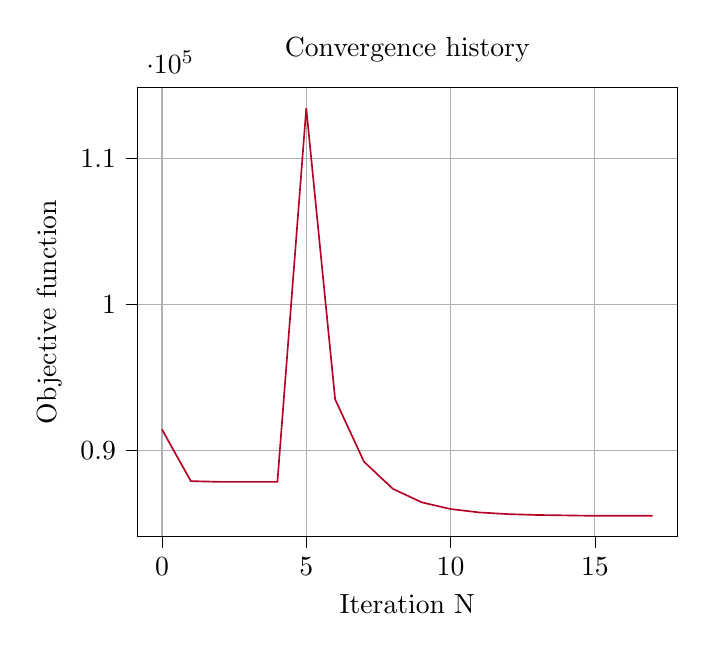
\begin{tikzpicture}

\definecolor{darkgray176}{RGB}{176,176,176}
\definecolor{firebrick180438}{RGB}{180,4,38}

\begin{axis}[
tick align=outside,
tick pos=left,
title={Convergence history},
x grid style={darkgray176},
xlabel={Iteration N},
xmajorgrids,
xmin=-0.85, xmax=17.85,
xtick style={color=black},
y grid style={darkgray176},
ylabel={Objective function},
ymajorgrids,
ymin=84140.4973908178, ymax=114805.744111147,
ytick style={color=black}
]
\addplot [semithick, firebrick180438]
table {%
0 91442.5585116738
1 87907.0802673692
2 87857.9447685309
3 87857.9100270034
4 87857.9100269807
5 113411.869260223
6 93505.0018496608
7 89235.3746151231
8 87381.5440623512
9 86457.9648560041
10 85996.1760131869
11 85765.281682217
12 85649.8296002172
13 85592.1081534132
14 85563.2480255216
15 85534.3722417418
16 85534.3878951324
17 85534.3878951312
};
\end{axis}

\end{tikzpicture}
